\PassOptionsToPackage{unicode=true}{hyperref} % options for packages loaded elsewhere
\PassOptionsToPackage{hyphens}{url}
%
\documentclass{book}        % from not too short p76 pagestyle
%\usepackage{fancyhdr}
%\pagestyle{fancy}
%ensure chapter section headngs in lower case
%
\usepackage{graphicx}
\DeclareGraphicsExtensions{.png,.jpg}
\usepackage{xeCJK}
\setCJKmainfont{SimSun}
\usepackage{lmodern}
\usepackage{amssymb,amsmath}
\usepackage{ifxetex,ifluatex}
\usepackage{fixltx2e} % provides \textsubscript
\ifnum 0\ifxetex 1\fi\ifluatex 1\fi=0 % if pdftex
  \usepackage[T1]{fontenc}
  \usepackage[utf8]{inputenc}
  \usepackage{textcomp} % provides euro and other symbols
\else % if luatex or xelatex
  \usepackage{unicode-math}
  \defaultfontfeatures{Ligatures=TeX,Scale=MatchLowercase}
\fi
% use upquote if available, for straight quotes in verbatim environments
\IfFileExists{upquote.sty}{\usepackage{upquote}}{}
% use microtype if available
\IfFileExists{microtype.sty}{%
\usepackage[]{microtype}
\UseMicrotypeSet[protrusion]{basicmath} % disable protrusion for tt fonts
}{}
\IfFileExists{parskip.sty}{%
\usepackage{parskip}
}{% else
\setlength{\parindent}{0pt}
\setlength{\parskip}{6pt plus 2pt minus 1pt}
}
\usepackage{hyperref}
\hypersetup{
            pdfborder={0 0 0},
            breaklinks=true}
\urlstyle{same}  % don't use monospace font for urls
\usepackage{longtable,booktabs}
% Fix footnotes in tables (requires footnote package)
\usepackage{multirow} %for tabular combine multirow
\IfFileExists{footnote.sty}{\usepackage{footnote}\makesavenoteenv{longtable}}{}
\setlength{\emergencystretch}{3em}  % prevent overfull lines
\providecommand{\tightlist}{%
  \setlength{\itemsep}{0pt}\setlength{\parskip}{0pt}}
\setcounter{secnumdepth}{0}
% Redefines (sub)paragraphs to behave more like sections
\ifx\paragraph\undefined\else
\let\oldparagraph\paragraph
\renewcommand{\paragraph}[1]{\oldparagraph{#1}\mbox{}}
\fi
\ifx\subparagraph\undefined\else
\let\oldsubparagraph\subparagraph
\renewcommand{\subparagraph}[1]{\oldsubparagraph{#1}\mbox{}}
\fi

% set default figure placement to htbp
\makeatletter
\def\fps@figure{htbp}
\makeatother
\date{}

\usepackage{graphicx}

\raggedbottom

\begin{document}




\resizebox{\linewidth}{!}{

\renewcommand{\arraystretch}{1.5}

\begin{tabular}{|c|c|c|}
\hline
\:&Conventional传统分工&Composite自主团队\\
\hline
\multicolumn{3}{|c|}{Absenteeism (\% of possible shifts)旷工率(可能轮班数之百分比) }\\
\hline
Without reason 没有理由&4.3&0.4 \\
\hline
Sickness or other 病或其他&8.9&4.6\\
\hline
Accidents 意外&6.8&3.2\\
\hline
Total 总数&20.0&8.2\\
\hline
\end{tabular}

}




























\resizebox{\linewidth}{!}{

\renewcommand{\arraystretch}{1.5}

\begin{tabular}{|c|c|c|}
\hline
估算步骤&专家估算&模型\\
\hline
评判不同信息的比重&主观判断&基于对历史数据的统计分析\\
\hline
从信息估算工作量&主观判断&基于正式重复性的过程和方程式 \\
\hline
回顾/讨论工作量估算/主观判断+分析过程，参考检查单、指南和专家意见&主观判断+分析过程，参考检查单、指南和专家意见，可能再主观判断更新工作量估算 \\
\hline
\end{tabular}

}


\resizebox{\linewidth}{!}{ 

\renewcommand{\arraystretch}{1.5}

\begin{tabular}{|c|c|c|}
\hline
\:&Conventional传统分工&Composite自主团队\\
\hline
Number of men人数&41&41\\
\hline
Number of segregated tasks 任务数&14&1 \\
\hline
\multirow{3}{*}{Mean job variation for members 每成员的平均任务/变化数: }\\
\hline
Tasks work with 要处理的任务:&1.0&5.5\\
\hline
Main tasks worked 主要任务:&1.0&3.6\\
\hline
Diff. shifts worked 不同的轮班:&2.0&2.9\\
\hline
\end{tabular}

}


从下面表2可以看到右面的组织架构更灵活，生产率比传统的单一工作设计高。右面的自主团队架构更能适应变化万千的采矿、采煤环境。采煤的步骤安排，也必须按照按环境的不同来应对。但如果是左面的硬性单一分工安排，缺乏这种灵活性（除非是专业性强的技术工种，必须把工作细分,每个人做某一件事)。但在采煤机械化、批量生产这种技术没有这个限制，所以采煤工人经过一些学习可以兼任其他工作。

%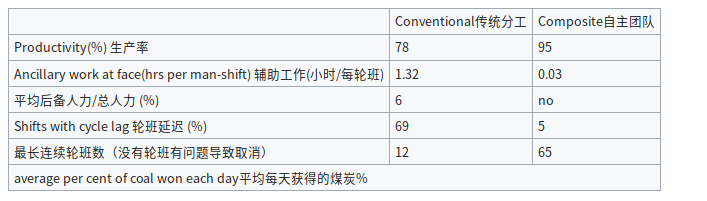
\includegraphics[width=10cm]{Screenshotfrom2023-11-0303-25-45.png}



\resizebox{\linewidth}{!}{

\renewcommand{\arraystretch}{1.5}


\begin{tabular}{|c|c|c|}
\hline
\:&Conventional传统分工&Composite自主团队\\
\hline
Productivity(\%) 生产率&78&95\\
\hline
Ancillary work at face(hrs per man-shift) 辅助工作(小时/每轮班)&1.32&0.03 \\
\hline
平均后备人力/总人力 (\%)&6&no\\
\hline
Shifts with cycle lag 轮班延迟 (\%)&69&5\\
\hline
最长连续轮班数（没有轮班有问题导致取消）&12&65\\
\hline
\multirow{3}{*}{average per cent of coal won each day平均每天获得的煤炭\%}\\
\hline
\end{tabular}

}


团队组织架构除了让工人更好做好采矿工作以外，也可以更好满足工人的个人心理需要，包括互相支持，有团队合作的概念。但是如果按左面传统的工业化分工，就缺乏合作。导致很多采煤工只能单打独斗，孤立无援，导致心理压力很大。这个也可以从表3的缺勤率看得出来，会更容易无缘无故请假等，背后主因是分工设计导致工人心理压力太大，承受不了。团队互相协助的环境可以减轻这方面的压力。

%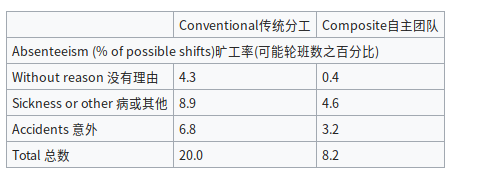
\includegraphics[width=10cm]{Screenshotfrom2023-11-0303-26-09.png}

\resizebox{\linewidth}{!}{

\renewcommand{\arraystretch}{1.5}

\begin{tabular}{|c|c|c|}
\hline
\:&Conventional传统分工&Composite自主团队\\
\hline
\multirow{3}{*}{Absenteeism (\% of possible shifts)旷工率(可能轮班数之百分比) }\\
\hline
Without reason 没有理由&4.3&0.4 \\
\hline
Sickness or other 病或其他&8.9&4.6\\
\hline
Accidents 意外&6.8&3.2\\
\hline
Total 总数&20.0&8.2\\
\hline
\end{tabular}

}

\vspace{10mm} 

我们继续看，发现3月有异常点，后面在5月份也有异常点。如果我们再看后面月份的逆差数据，看见明显比前面降低。\\
%\href{文件:The_key_fig2.11.1.1.png}{450px}

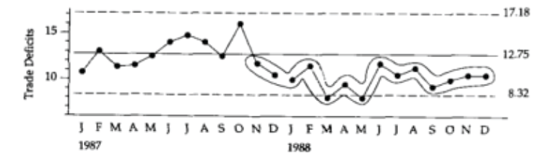
\includegraphics[width=10cm]{The_key_fig21111.png}

\vspace{-2mm} 

客户：理解了。这个对于我们定基线有什么作用啊？\\
我：从刚才贸易逆差的数据，我们就不能把两年的数据的均值与范围（极差）作为基线，应该是以后面降低后的那些点，才能真正反应当前的水平和分布。

\vspace{-2mm} 

如果不是工业生产，不一定有这么多数据去随机抽样、求均值，怎么办呢？可以用ImR图
(或
XmR)，比如下图就是某个医院做外科心脏手术所花的时间的统计，想看看开心手术的时间是否稳定，因为外科手术特别危险，越长时间那个患者的存活机会就越低，也看到是有异常点。

%\href{文件:控制图08.1.png}{500px}

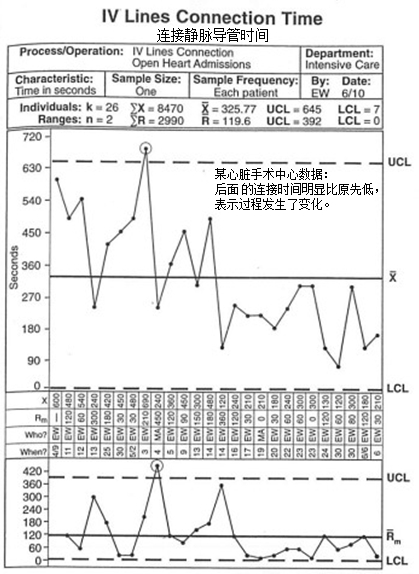
\includegraphics[width=10cm]{357替换图片.png}

（ImR 控制图相关公式，详见附件）

%\vfill 

%\vspace{} \vfill 

\end{document}
